% ============================================================
% KAPITEL 6 — EVALUATION
% ============================================================

\chapter{Evaluation}
\label{ch:evaluation}

Dieses Kapitel vergleicht die Repräsentationsformen entlang einer nach Referenztypen aufgeschlüsselten Taxonomie und bestimmt, welche Form welche Art von Referenz trägt (RQ1).
Anschließend prüft es, ob sich die hybride Repräsentation allein über ihre Instruktion so gestalten lässt, dass sie die Stärken beider Schichten vereint (RQ2).
Zum Schluss werden Validität und Grenzen der Ergebnisse diskutiert.


% ------------------------------------------------------------
\section{Evaluationsdesign}
\label{sec:eval-design}

Verglichen werden die fünf Varianten aus Abschnitt~\ref{sec:impl-variants}.
Sie nutzen dieselben Szenen, Befehle und Manipulationswerkzeuge und unterscheiden sich allein darin, in welcher Form die Szene dem Agenten bereitgestellt wird.
Da alle Varianten Objekte über dasselbe Kennungssystem ansprechen (Abschnitt~\ref{sec:konz-fairness}), gehen gemessene Unterschiede nicht auf einen ungleichen Werkzeugzugriff zurück.
Für die Deutung ist dabei im Blick zu behalten, dass das entscheidende Sprachmodell in keiner Variante ein Bild erhält, sondern im visuellen Fall eine Beschreibung des Bildes (Abschnitt~\ref{sec:grundlagen-modelle}).
Streng genommen werden also eine exakte Datenstruktur und eine unscharfe sprachliche Beschreibung derselben Szene verglichen.

Ob eine Manipulation gelungen ist, wird aus dem tatsächlichen Zustand der Szene nach der Ausführung bestimmt, den die Auswertung mit der Soll-Vorgabe des Szenarios vergleicht (Abschnitt~\ref{sec:eval-metrics}).
Die Selbstauskunft des Agenten bleibt unberücksichtigt, weil das lokale Modell wiederholt Erfolge meldete, die der Folgezustand nicht bestätigte (Abschnitt~\ref{sec:eval-validity}).

Jede Kombination aus Szenario und Variante wird zehnmal ausgeführt und der gesamte Durchlauf dreimal wiederholt, sodass jede Zelle auf 30 Läufen beruht.
Berichtet wird der Mittelwert über die drei Durchläufe mit der Spanne von Minimum und Maximum, an der sich ablesen lässt, wie stark eine Zelle zwischen den Durchläufen schwankt.
Für die zentralen Vergleiche werden die 30 Läufe einer Zelle zusätzlich zusammengefasst und inferenzstatistisch ausgewertet.

Ausgewertet werden dreizehn Szenarien in fünf Kategorien.
Die Kategorien A, B und C umfassen je drei Szenarien, D und E nur je zwei, obwohl gerade diese beiden die inhaltlich zentralen Befunde tragen.
Die Szenen bestehen aus einfachen geometrischen Grundkörpern und sind so aufgebaut, dass jedes Szenario eine bestimmte Repräsentationskompetenz isoliert.
Gemessen wird am Desktop, weil sich die Szenen dort exakt kontrollieren und beliebig oft identisch wiederholen lassen; die immersive Umgebung ist nur Zielumgebung des Demonstrators.
Als Sprachmodell dient Qwen2.5-7B, als visuelles Modell Qwen2.5-VL-7B, beide selbst gehostet und gemeinsam auf einer NVIDIA RTX A5000 mit 24 Gigabyte Grafikspeicher.
Tabelle~\ref{tab:config} führt die vollständige Konfiguration auf, die nach NFA3 für eine Wiederholung der Messung nötig ist.

\begin{table}[htbp]
  \centering
  \caption{Konfiguration der Messung, beschränkt auf die Angaben, die den
           Ausgang der Läufe beeinflussen. Zusammen mit dem verlinkten Code
           genügen sie, um die Messung zu wiederholen.}
  \label{tab:config}
  \small
  \setlength{\tabcolsep}{5pt}
  \renewcommand{\arraystretch}{1.3}
  \begin{tabular}{@{}p{3.4cm} p{9.6cm}@{}}
    \toprule
    Größe & Wert \\
    \midrule
    Sprachmodell      & \texttt{qwen2.5-7b-instruct}, GGUF Q4\_K\_M, 4096 Token Kontext \\
    Visuelles Modell  & \texttt{qwen/qwen2.5-vl-7b}, GGUF Q4\_K\_M, 4096 Token Kontext \\
    Hardware, Laufzeit & NVIDIA RTX A5000 mit 24\,GB, LM Studio (CLI-Commit \texttt{efce996}), beide Modelle gleichzeitig geladen \\
    Agent             & smolagents 1.26.0 (\texttt{ToolCallingAgent}) unter Python 3.13, \texttt{max\_steps} = 6 \\
    Dekodierung       & Sprachmodell: Temperatur 0{,}8 (Voreinstellung der Laufzeitumgebung, im Client nicht überschrieben). Visuelles Modell: Temperatur 0{,}1 (im Client ausdrücklich gesetzt). Kein fester Seed \\
    Messumfang        & 13 Szenarien $\times$ 5 Varianten, je 10 Läufe in 3 Durchläufen, also 30 Läufe pro Zelle \\
    Code und Rohdaten & \url{https://git.informatik.fh-nuernberg.de/jobboerse/forschung/bachelorarbeiten/bachelorarbeit-sandro-jaeger} \\
    \bottomrule
  \end{tabular}
\end{table}

Beide Modelle liegen in derselben Quantisierungsstufe vor.
Eine unterschiedlich starke Quantisierung hätte die beiden Schichten ungleich beeinträchtigt und damit neben der Repräsentationsform eine weitere Störgröße eingeführt.
Mit 4{,}68\,GB und 6{,}04\,GB belegen die Gewichte zusammen rund 10{,}7\,GB, sodass auf der Karte Platz für den Schlüssel-Wert-Zwischenspeicher beider Modelle bleibt; erst dadurch ist der gleichzeitige Betrieb nach NFA2 möglich.

Knapp bemessen ist dagegen die Kontextlänge von 4096 Token, und sie trifft die Varianten ungleich.
Zusätzlich zu Grundinstruktion, Werkzeugbeschreibungen und bisherigem Verlauf der Agentenschleife trägt die strukturelle Variante nur den JSON-Zustand im Kontext, die visuelle nur die Beschreibung, die hybriden Varianten aber beides.
Für mehrere aufeinanderfolgende Schritte bleibt ihnen deshalb systematisch weniger Platz.
Ob sich das in den Messungen auswirkte, etwa durch abgeschnittenen Kontext in längeren Läufen, wurde nicht überwacht und lässt sich nachträglich nicht mehr feststellen.

Unterschiedlich ist auch die Dekodierung der beiden Modelle.
Das Sprachmodell, das die Entscheidung trifft, lief mit einer Temperatur von 0{,}8, einer Einstellung, die den Antwortraum spürbar öffnet.
Die zehn Läufe einer Zelle sind damit weitgehend unabhängige Ziehungen aus einer breiten Verteilung und keine Wiederholungen derselben Antwort.
Eine Zelle, die bei 0 von 30 oder bei 30 von 30 liegt, kommt also nicht dadurch zustande, dass das Modell ohnehin immer dasselbe antwortet, sondern trotz des Spielraums in der Dekodierung.
Die vielen Zellen ohne Streuung sind unter dieser Bedingung ein Befund und kein Artefakt einer zu niedrigen Temperatur: Der jeweilige Effekt wirkt stärker als das Rauschen.

Das visuelle Modell lief dagegen mit einer Temperatur von 0{,}1 und damit nahezu deterministisch, sodass die Beschreibung einer gegebenen Szene über die Läufe hinweg weitgehend gleich ausfällt.
Das ist gewollt, denn die Wahrnehmungsstufe ist Eingabe und nicht Untersuchungsgegenstand, und eine stark schwankende Beschreibung hätte eine zusätzliche Störgröße zwischen Repräsentationsform und Ergebnis geschoben.
Die Streuung einer Zelle geht damit fast vollständig auf das Sprachmodell zurück, also auf die Stufe, die verglichen wird.
Eine Restabhängigkeit zwischen den Läufen bleibt, weil alle Läufe einer Zelle dieselbe, nahezu unveränderliche Szenenbeschreibung nutzen; sie betrifft aber die Eingabe und nicht die gemessene Entscheidung.


% ------------------------------------------------------------
\section{Referenztyp-Taxonomie}
\label{sec:eval-taxonomy}

Welche Repräsentation eine Aufgabe trägt, hängt davon ab, worauf sich der Befehl bezieht.
Ein Verweis auf die Farbe eines Objekts stellt andere Anforderungen als ein Verweis auf seine Lage oder auf ein Objekt, das im Bild gar nicht zu sehen ist.
Eine pauschale Antwort auf die Frage nach der besten Repräsentation gibt es deshalb nicht.
Die Evaluation zerlegt die natürlichsprachliche Referenz stattdessen in fünf Typen und prüft für jeden einzeln, welche Repräsentation ihn auflösen kann.
Tabelle~\ref{tab:taxonomy} zeigt, in welcher Schicht die dafür nötige Information jeweils verfügbar ist.

Kategorie A ist die Kontrollbedingung.
Der Befehl benennt das Zielobjekt direkt über seine Kennung, sodass die Aufgabe unabhängig von der Repräsentationsform lösbar ist; sie prüft also den Messaufbau und vergleicht nicht inhaltlich.
In Kategorie B wird ein Objekt über ein Attribut wie Farbe oder Größe angesprochen, in Kategorie C über eine räumliche Relation zu einem anderen Objekt, etwa \enquote{links von}.
Bei beiden lässt sich das gemeinte Objekt aus Eigenschaften oder Koordinaten bestimmen, die in den strukturellen Daten stehen.

Die Kategorien D und E bilden das eigentliche Gegensatzpaar.
In D bezieht sich der Befehl auf eine rein perzeptuelle Eigenschaft, etwa ein Oberflächenmuster, das in den strukturellen Daten nicht vorkommt; das Objekt lässt sich nur über das Bild bestimmen.
In E ist das Objekt im Bild verdeckt, in den strukturellen Daten aber vollständig verzeichnet, sodass es sich nur über die Struktur bestimmen lässt.
An diesen beiden Polen hat jeweils nur eine Schicht Zugang zur Antwort, und an ihnen zeigt sich, ob eine Repräsentation eine Kompetenz besitzt, die der anderen grundsätzlich fehlt.

Die Unterscheidung nach Referenztypen knüpft an bestehende Arbeiten an, die Referenzen etwa nach ihrer Abhängigkeit vom Blickwinkel oder nach der Eindeutigkeit des Zielobjekts einteilen~\cite{achlioptas2020, chen2020}.
Neu sind in der vorliegenden Taxonomie die rein perzeptuelle und die verdeckte Referenz als eigene Typen, ohne die sich die exklusiven Zuständigkeiten der beiden Repräsentationen nicht prüfen ließen.
Tabelle~\ref{tab:scenarios} führt die konkreten Szenarien je Referenztyp auf.

\begin{table}[ht]
  \centering
  \caption{Verfügbarkeit der zur Auflösung nötigen Information je Referenztyp und Schicht, nach Konstruktion der Szenarien. Die Zeilen D und E bilden das exklusive Gegensatzpaar.}
  \label{tab:taxonomy}
  \small
  \setlength{\tabcolsep}{5pt}
  \renewcommand{\arraystretch}{1.3}
  \begin{tabular}{@{}p{2.9cm} p{5.1cm} p{5.1cm}@{}}
    \toprule
    Referenztyp & In der strukturellen Schicht & In der visuellen Schicht \\
    \midrule
    A — direkt        & Kennung und Zielkoordinaten vorhanden & markiertes Objekt sichtbar \\
    B — Attribut      & Attribute wie Farbe und Größe vorhanden & Aussehen sichtbar \\
    C — relational    & exakte Koordinaten vorhanden & Anordnung sichtbar \\
    D — perzeptuell   & nicht enthalten & Muster sichtbar \\
    E — verdeckt      & vollständig verzeichnet & verdeckt, nicht sichtbar \\
    \bottomrule
  \end{tabular}
\end{table}

\begin{table}[htbp]
  \centering
  \caption{Übersicht aller ausgewerteten Szenarien mit Befehl, Ausgangsszene und Soll-Ergebnis. Die Befehle geben den real gesendeten englischen Stimulus wieder.}
  \label{tab:scenarios}
  \footnotesize
  \setlength{\tabcolsep}{4pt}
  \renewcommand{\arraystretch}{1.2}
  \begin{tabular}{@{}p{0.6cm} p{3.6cm} p{4.4cm} p{3.6cm}@{}}
    \toprule
    ID & Befehl & Ausgangsszene & Soll-Ergebnis \\
    \midrule
    \multicolumn{4}{@{}l}{\textit{Kategorie A — direkt / id-basiert}} \\
    A1 & \enquote{Spawn a red cube at x=2, y=0, z=1.} & leere Szene & roter Würfel bei (2,0,1) vorhanden \\
    A2 & \enquote{Move obj\_2 to position (0, 1, 0).} & rot (0,0,0), grün (2,0,0), blau (4,0,0) & grüner Würfel (obj\_2) bei (0,1,0) \\
    A3 & \enquote{Delete obj\_1.} & wie A2 & roter Würfel (obj\_1) entfernt \\
    \addlinespace
    \multicolumn{4}{@{}l}{\textit{Kategorie B — Attribut-Referenz}} \\
    B1 & \enquote{Raise the red cube by 1 unit.} & rot (1,0,0), blau (3,0,0) & roter Würfel in der Höhe +1 \\
    B2 & \enquote{Delete all red cubes.} & rot (0,0,0), rot (2,0,0), grüne Kugel (4,0,0) & beide roten Würfel entfernt, Kugel bleibt \\
    B3 & \enquote{Move the largest object to (0, 0, 0).} & roter Würfel Größe 0,5 (-2,0,0); grüner Größe 1,5 (0,0,3); blauer Größe 1,0 (3,0,0) & größtes Objekt (grün) bei (0,0,0) \\
    \addlinespace
    \multicolumn{4}{@{}l}{\textit{Kategorie C — räumlich-relational}} \\
    C1 & \enquote{Move the sphere to the left of the cube.} & blaue Kugel (1,0,0), grüner Würfel (-1,0,0) & Kugel links vom Würfel \\
    C2\,$^{a}$ & \enquote{Raise the cube nearest to the camera by 1.} & rot (-2,0,2), grün (0,0,5), blau (2,0,8) & kamera-nächster Würfel in der Höhe +1 \\
    C4 & \enquote{Place the sphere exactly 2 units left of the cube.} & grüner Würfel (1,0,0), blaue Kugel (4,0,0) & Kugel bei x=-1 (genau 2 links) \\
    \addlinespace
    \multicolumn{4}{@{}l}{\textit{Kategorie D — rein perzeptuell}} \\
    D1 & \enquote{Raise the striped cube by 1 unit.} & zwei graue Würfel (-1,0,3) und (1,0,3); zweiter gestreift & gestreifter Würfel +1, anderer unverändert \\
    D2 & \enquote{Move the most salient object to (0, 0, 0).} & vier graue Würfel (-3/-1/3/5, 0, 4); ein gestreifter (1,0,4) & gestreifter (auffälliger) Würfel bei (0,0,0) \\
    \addlinespace
    \multicolumn{4}{@{}l}{\textit{Kategorie E — verdeckt}} \\
    E1 & \enquote{Raise the green cube by 1 unit.} & rot (-3,0,5); graue Wand Größe 4,0 (2,0,2); grün (2,0,6) dahinter verdeckt & verdeckter grüner Würfel +1 \\
    E2 & \enquote{Raise every cube by 1 unit.} & wie E1 & alle drei Würfel in der Höhe +1 \\
    \bottomrule
  \end{tabular}

  \vspace{2mm}
  {\footnotesize
  \begin{minipage}{0.97\linewidth}
  Positionen als (x,\,y,\,z), wobei y die Höhe angibt. \enquote{Größe} ist die relative Kantenlänge (Standard 1,0).\\[2pt]
  $^{a}$~C2 mit seitlich versetztem Aufbau. Der ursprünglich achsenkollineare Aufbau wurde ersetzt (Abschnitt~\ref{sec:eval-validity}). Szenario C3 wurde aus methodischen Gründen ausgeschlossen (ebenda).
  \end{minipage}}
\end{table}


% ------------------------------------------------------------
\section{Metriken}
\label{sec:eval-metrics}

Die Erfolgs- und Genauigkeitsmaße orientieren sich an etablierten Metriken aus der Literatur zum sprachlichen Auffinden von Objekten in 3D-Szenen~\cite{chen2020, achlioptas2020}.
Primäre Kennzahl ist der Ausführungserfolg.
Er ist je Lauf binär und ergibt sich allein aus dem Folgezustand der Szene, den die Auswertung nach der Manipulation mit der Soll-Vorgabe des Szenarios vergleicht.
Berichtet wird die Zahl der Erfolge aus zehn Läufen, gemittelt über die drei Durchläufe mit der zugehörigen Spanne.

Was als erfüllte Vorgabe gilt, hängt vom Aufgabentyp ab.
In jedem Fall muss das richtige Objekt betroffen sein: Wird ein anderes als das gemeinte Objekt verändert, ist der Lauf ein Misserfolg, auch wenn die Zielkoordinate sonst getroffen wäre.
Dieses Kriterium erfasst, ob die Referenz korrekt aufgelöst wurde.
Bei Aufgaben mit Zielposition muss außerdem die erreichte Position innerhalb einer festen Toleranz $\tau$ um den Sollwert liegen.
Bei relationalen Aufgaben muss die geforderte Lagebeziehung im Folgezustand gelten, etwa dass ein Objekt einen kleineren x-Wert besitzt als ein anderes, und beim Entfernen oder Erzeugen muss das Objekt im Folgezustand fehlen beziehungsweise vorhanden sein.
Ein Lauf zählt nur als Erfolg, wenn das jeweils maßgebliche Kriterium vollständig erfüllt ist.

Die Toleranz ist auf $\tau = 0{,}1$ Einheiten gesetzt.
Sie ist nicht aus einer externen Vorgabe übernommen, sondern für diesen Aufbau festgelegt und an zwei Größen ausgerichtet.
Sie liegt deutlich unter der kleinsten in den Szenarien geforderten Verschiebung von einer Einheit, sodass eine grob danebenliegende Bewegung nicht als Treffer zählt, und über der Genauigkeit, mit der die Engine Positionen zurückmeldet, sodass numerisches Rauschen keinen korrekten Lauf verwirft.
Ein Zehntel der kleinsten geforderten Distanz erfüllt beides.
Wie empfindlich die Ergebnisse auf diese Wahl reagieren, wurde nicht untersucht.

Einen kontinuierlichen Lagefehler, also den Abstand zwischen erreichter und geforderter Position, berichtet die Arbeit nicht; $\tau$ geht nur als Schwelle in das binäre Kriterium ein.
Nachträglich lässt er sich auch nicht mehr berechnen, weil für die metrischen Szenarien C2 und C4 die erreichten Endpositionen nicht mehr vorliegen.
Das ist bedauerlich, denn gerade dort scheitern alle Varianten am binären Kriterium, und erst der Lagefehler würde zeigen, ob sie knapp danebenliegen oder die Aufgabe grundsätzlich verfehlen.

\subsection*{Statistische Auswertung}

Mittelwert und Spanne über drei Durchläufe beschreiben, wie stabil eine Zelle ist, taugen als Entscheidungsgrundlage aber nur begrenzt.
Drei Durchläufe sind eine schmale Basis, und nicht überlappende Spannen als belastbar zu werten, wäre eine Heuristik ohne Fehlerkontrolle.
Für die inhaltlich zentralen Vergleiche werden deshalb die je 30 Einzelläufe einer Zelle zusammengefasst und inferenzstatistisch ausgewertet.

Da jeder Lauf binär ausgeht, ist eine Zelle durch die Zahl $k$ der Erfolge aus $n = 30$ Läufen vollständig beschrieben.
Für jede Zelle wird die Erfolgsrate $k/n$ mit einem Wilson-Konfidenzintervall zum Niveau 95\,\% angegeben.
Das Wilson-Intervall ist hier dem Normalapproximationsintervall vorzuziehen, weil viele Zellen bei null oder bei allen Erfolgen liegen, wo die Normalapproximation ein Intervall der Breite null liefern würde.
Zwei Zellen werden mit dem exakten Test nach Fisher auf der zugehörigen Vierfeldertafel verglichen, der keine Annahmen über erwartete Zellhäufigkeiten voraussetzt und auch bei extremen Anteilen gültig bleibt.

Die dafür nötige Annahme unabhängiger Läufe ist wegen der in Abschnitt~\ref{sec:eval-design} beschriebenen Dekodierung im Wesentlichen erfüllt.
Das Niveau wird nicht für multiples Testen korrigiert.
Die zentralen Unterschiede sind allerdings so groß, dass keiner an einer Entscheidungsgrenze liegt; die schwächsten Vergleiche, die beiden in D2 mit $p = 0{,}0046$, blieben auch bei einer konservativen Korrektur bestehen.


% ------------------------------------------------------------
\section[Ergebnisse zu RQ1]{Ergebnisse zum Einfluss der Repräsentationsform (RQ1)}
\label{sec:eval-rq1}

Tabelle~\ref{tab:results-scenario} zeigt die Ergebnisse je Szenario als Mittelwert über drei Durchläufe mit der Spanne [Minimum--Maximum], wobei jede Zelle für zehn mögliche Erfolge steht.
Tabelle~\ref{tab:results-category} fasst diese Werte je Kategorie zusammen.
Die Tabellen~\ref{tab:stats} und~\ref{tab:fisher} enthalten keine zusätzlichen Messungen, sondern fassen die inhaltlich tragenden Zellen als Erfolge aus je 30 Läufen mit Wilson-Konfidenzintervall zusammen und geben die exakten Tests für die Vergleiche an, auf denen die Argumentation dieses und des folgenden Abschnitts beruht.

% Werte: Mittelwert [Min--Max] ueber 3 Durchlaeufe, je 10 moegliche Erfolge.
% (1) C2 = separat neu gemessener, entkonfundierter Wert (siehe Validitaet).
% (2) E2 = kein reiner Verdeckungstest (Mehrschritt-Confound, siehe Validitaet).
\begin{table}[ht]
  \centering
  \caption{Erfolg je Szenario und Variante: Mittelwert [Min--Max] über drei
           Durchläufe (je $N=10$).}
  \label{tab:results-scenario}
  \footnotesize
  \setlength{\tabcolsep}{4pt}
  \begin{tabular}{c l ccccc}
    \toprule
    Kat. & Szen. & json & vlm & hybrid & guided & surgical \\
    \midrule
    A & A1 & 10{,}0 [10--10] & 10{,}0 [10--10] & 10{,}0 [10--10] & 10{,}0 [10--10] & 10{,}0 [10--10] \\
    A & A2 & 10{,}0 [10--10] & 10{,}0 [10--10] & 10{,}0 [10--10] & 10{,}0 [10--10] & 10{,}0 [10--10] \\
    A & A3 & 10{,}0 [10--10] & 10{,}0 [10--10] & 10{,}0 [10--10] & 10{,}0 [10--10] & 10{,}0 [10--10] \\
    B & B1 & 10{,}0 [10--10] & 10{,}0 [10--10] & 10{,}0 [10--10] & 10{,}0 [10--10] & 10{,}0 [10--10] \\
    B & B2 & 10{,}0 [10--10] &  9{,}7 [9--10]  & 10{,}0 [10--10] & 10{,}0 [10--10] & 10{,}0 [10--10] \\
    B & B3 & 10{,}0 [10--10] &  0{,}0 [0--0]   & 10{,}0 [10--10] & 10{,}0 [10--10] & 10{,}0 [10--10] \\
    C & C1 & 10{,}0 [10--10] &  1{,}7 [0--3]   &  8{,}3 [7--10]  & 10{,}0 [10--10] & 10{,}0 [10--10] \\
    C & C2\textsuperscript{(1)} & 0{,}0 [0--0] & 0{,}0 [0--0] & 0{,}3 [0--1] & 2{,}7 [1--4] & 2{,}0 [1--3] \\
    C & C4 &  1{,}7 [0--4]  &  0{,}7 [0--2]   &  3{,}3 [3--4]   &  1{,}3 [1--2]  &  2{,}0 [1--3]  \\
    D & D1 &  0{,}0 [0--0]  & 10{,}0 [10--10] &  0{,}7 [0--1]   &  8{,}3 [6--10] &  9{,}7 [9--10] \\
    D & D2 &  0{,}3 [0--1]  & 10{,}0 [10--10] & 10{,}0 [10--10] &  7{,}3 [6--9]  & 10{,}0 [10--10] \\
    E & E1 & 10{,}0 [10--10] &  0{,}0 [0--0]   & 10{,}0 [10--10] & 10{,}0 [10--10] & 10{,}0 [10--10] \\
    E & E2\textsuperscript{(2)} & 10{,}0 [10--10] & 0{,}0 [0--0] & 0{,}3 [0--1] & 0{,}0 [0--0] & 0{,}0 [0--0] \\
    \bottomrule
  \end{tabular}

  \vspace{2mm}
  {\footnotesize
  \begin{minipage}{0.97\linewidth}
  Spaltenköpfe sind die Kurzformen der Varianten nach Tabelle~\ref{tab:variants}:
  \texttt{json} strukturell, \texttt{vlm} visuell, \texttt{hybrid} naiv hybrid,
  \texttt{guided} priorisierend, \texttt{surgical} kompetenzgetrennt.\\[2pt]
  \textsuperscript{(1)}~C2 wurde nach Entdeckung eines Störfaktors mit seitlich
  versetztem Aufbau neu gemessen; die Werte stammen aus dieser zweiten Messung
  und sind nicht mit den übrigen Zeilen im selben Durchlauf erhoben
  (Abschnitt~\ref{sec:eval-validity}).\\[2pt]
  \textsuperscript{(2)}~E2 ist kein reiner Verdeckungstest. Das Soll-Ergebnis
  verlangt die Manipulation mehrerer Objekte und damit mehr als einen
  Manipulationsaufruf, was der Grundinstruktion widerspricht
  (Abschnitt~\ref{sec:eval-validity}). Die Zeile wird deshalb nicht als
  Repräsentationsbefund gewertet.
  \end{minipage}}
\end{table}

\begin{table}[ht]
  \centering
  \caption{Erfolg je Kategorie als Summe der zugehörigen Szenario-Mittelwerte
           über drei Durchläufe. Eine Spanne wird hier nicht ausgewiesen, da
           sich Minimum und Maximum einer Kategorie nicht aus den
           Szenario-Spannen zusammensetzen lassen. Kategorie E getrennt
           ausgewiesen.}
  \label{tab:results-category}
  \small
  \setlength{\tabcolsep}{4pt}
  \begin{tabular}{l c ccccc}
    \toprule
    Kat. & max & json & vlm & hybrid & guided & surgical \\
    \midrule
    A          & 30 & 30{,}0 & 30{,}0 & 30{,}0 & 30{,}0 & 30{,}0 \\
    B          & 30 & 30{,}0 & 19{,}7 & 30{,}0 & 30{,}0 & 30{,}0 \\
    C          & 30 & 11{,}7 &  2{,}4 & 11{,}9 & 14{,}0 & 14{,}0 \\
    D          & 20 &  0{,}3 & 20{,}0 & 10{,}7 & 15{,}6 & 19{,}7 \\
    E1         & 10 & 10{,}0 &  0{,}0 & 10{,}0 & 10{,}0 & 10{,}0 \\
    E2         & 10 & 10{,}0 &  0{,}0 &  0{,}3 &  0{,}0 &  0{,}0 \\
    \bottomrule
  \end{tabular}
\end{table}

\begin{table}[ht]
  \centering
  \caption{Zentrale Zellen als Erfolge aus $n=30$ Läufen mit
           Wilson-95\,\%-Konfidenzintervall der Erfolgsrate.}
  \label{tab:stats}
  \small
  \setlength{\tabcolsep}{5pt}
  \renewcommand{\arraystretch}{1.2}
  \begin{tabular}{@{}l l c c@{}}
    \toprule
    Szen. & Variante & Erfolge & Wilson-95\,\%-KI \\
    \midrule
    D1 & strukturell       &  0/30 & [\,0{,}0\,\%; 11{,}4\,\%] \\
    D1 & visuell           & 30/30 & [88{,}6\,\%; 100{,}0\,\%] \\
    D1 & naiv hybrid       &  2/30 & [\,1{,}8\,\%; 21{,}3\,\%] \\
    D1 & priorisierend     & 25/30 & [66{,}4\,\%; 92{,}7\,\%] \\
    D1 & kompetenzgetrennt & 29/30 & [83{,}3\,\%; 99{,}4\,\%] \\
    \addlinespace
    D2 & strukturell       &  1/30 & [\,0{,}6\,\%; 16{,}7\,\%] \\
    D2 & visuell           & 30/30 & [88{,}6\,\%; 100{,}0\,\%] \\
    D2 & naiv hybrid       & 30/30 & [88{,}6\,\%; 100{,}0\,\%] \\
    D2 & priorisierend     & 22/30 & [55{,}6\,\%; 85{,}8\,\%] \\
    D2 & kompetenzgetrennt & 30/30 & [88{,}6\,\%; 100{,}0\,\%] \\
    \addlinespace
    E1 & strukturell       & 30/30 & [88{,}6\,\%; 100{,}0\,\%] \\
    E1 & visuell           &  0/30 & [\,0{,}0\,\%; 11{,}4\,\%] \\
    B3 & visuell           &  0/30 & [\,0{,}0\,\%; 11{,}4\,\%] \\
    C1 & visuell           &  5/30 & [\,7{,}3\,\%; 33{,}6\,\%] \\
    \addlinespace
    C2 & strukturell       &  0/30 & [\,0{,}0\,\%; 11{,}4\,\%] \\
    C2 & priorisierend     &  8/30 & [14{,}2\,\%; 44{,}4\,\%] \\
    C4 & strukturell       &  5/30 & [\,7{,}3\,\%; 33{,}6\,\%] \\
    C4 & naiv hybrid       & 10/30 & [19{,}2\,\%; 51{,}2\,\%] \\
    \bottomrule
  \end{tabular}
\end{table}

\begin{table}[ht]
  \centering
  \caption{Exakte Tests nach Fisher für die zentralen Vergleiche, jeweils
           $n=30$ je Gruppe. Das Niveau ist nicht für multiples Testen
           korrigiert.}
  \label{tab:fisher}
  \small
  \setlength{\tabcolsep}{5pt}
  \renewcommand{\arraystretch}{1.2}
  \begin{tabular}{@{}l l l@{}}
    \toprule
    Vergleich & Erfolge & $p$ \\
    \midrule
    D1: naiv hybrid vs.\ visuell            &  2/30 vs.\ 30/30 & $8{,}4\cdot10^{-15}$ \\
    D1: naiv hybrid vs.\ kompetenzgetrennt  &  2/30 vs.\ 29/30 & $2{,}3\cdot10^{-13}$ \\
    D1: naiv hybrid vs.\ priorisierend      &  2/30 vs.\ 25/30 & $1{,}4\cdot10^{-9}$ \\
    D2: priorisierend vs.\ naiv hybrid      & 22/30 vs.\ 30/30 & $0{,}0046$ \\
    D2: priorisierend vs.\ kompetenzgetrennt& 22/30 vs.\ 30/30 & $0{,}0046$ \\
    \addlinespace
    D1: strukturell vs.\ visuell            &  0/30 vs.\ 30/30 & $1{,}7\cdot10^{-17}$ \\
    E1: visuell vs.\ strukturell            &  0/30 vs.\ 30/30 & $1{,}7\cdot10^{-17}$ \\
    B3: visuell vs.\ strukturell            &  0/30 vs.\ 30/30 & $1{,}7\cdot10^{-17}$ \\
    C1: visuell vs.\ strukturell            &  5/30 vs.\ 30/30 & $5{,}5\cdot10^{-12}$ \\
    \bottomrule
  \end{tabular}
\end{table}

\subsection*{Kategorie A: Kontrollbedingung}

Bevor sich Unterschiede zwischen den Repräsentationen deuten lassen, muss feststehen, dass der Aufbau misst, was er messen soll.
In Kategorie A nennt der Befehl Zielobjekt und Zielkoordinaten direkt über die \texttt{id}, eine Deutung der Szene ist nicht nötig, und bei sauberem Aufbau darf die Repräsentationsform keinen Unterschied machen.
So ist es auch: Alle fünf Varianten lösen jedes der drei Szenarien in allen 30 Läufen.
Kennungssystem und Werkzeugzugriff erzeugen also für sich keine variantenspezifischen Unterschiede.
Abweichungen in den übrigen Kategorien lassen sich damit auf die Repräsentationsform zurückführen, soweit nicht die in Abschnitt~\ref{sec:eval-validity} genannten Restkonfundierungen greifen.

\subsection*{Kategorie B: Attribut-Referenzen}

In Kategorie B wird ein Objekt über eine Eigenschaft wie Farbe oder Größe angesprochen.
Bis auf die visuelle lösen alle Varianten jedes Szenario vollständig, die visuelle erreicht 19,7 von 30.
Die kleine Abweichung in B2 (9,7 von 10) liegt innerhalb der beobachteten Streuung; fast der gesamte Rückstand entsteht in B3.
Dort soll das größte Objekt bewegt werden, und die visuelle Variante scheitert in allen 30 Läufen, während alle übrigen alle 30 lösen ($p = 1{,}7\cdot10^{-17}$, Tabelle~\ref{tab:fisher}).

Eine perspektivische Erklärung läge nahe, da ein weiter entferntes Objekt im Bild kleiner wirkt, als es ist.
Sie wird hier aber nicht gebraucht, denn die Ursache liegt im Aufbau der Pipeline.
Das Sprachmodell erhält nur die Beschreibung des visuellen Modells, und der Wahrnehmungs-Prompt fordert darin Nummer, Form, Farbe, qualitative Lage und Textur an, aber keine Größe (Listing~\ref{lst:vlmprompt}).
Der visuellen Variante fehlt in B3 also nicht die Wahrnehmungsfähigkeit, sondern die Information, nach der gefragt wird, und unter dieser Bedingung ist ein vollständiges Scheitern zu erwarten.
Das Ergebnis sagt damit etwas über den Zuschnitt des Prompts aus und nichts über eine grundsätzliche Grenze visueller Repräsentationen.
Ein Prompt, der auch die Größe abfragt, hätte vermutlich anders abgeschnitten; geprüft wurde das nicht.
Für diesen Aufbau bleibt festzuhalten, dass eine Referenz auf die absolute Größe über die strukturelle Schicht zuverlässig und über die visuelle gar nicht aufgelöst wird.

\subsection*{Kategorie C: Räumlich-relationale Referenzen}

In Kategorie C wird ein Objekt in Bezug auf ein anderes ausgewählt oder platziert.
Über die Kategorie hinweg bricht die visuelle Variante mit 2,4 von 30 fast vollständig ein, während die strukturelle und die hybriden Varianten mit rund 12 bis 14 von 30 deutlich davor liegen.
Relationale Aufgaben brauchen exakte Koordinaten, und die stehen nur in der strukturellen Schicht.

Am klarsten zeigt das C1, wo die Kugel links vom Würfel platziert werden soll.
Gefordert ist nur die Richtung der Relation, also ein negativer x-Abstand zum Würfel, kein exakter Zielwert.
Die strukturelle und die hybriden Varianten lösen das zuverlässig oder weitgehend, die visuelle scheitert fast durchgehend.

C4 verschärft dieselbe Aufgabe zu einer metrischen Vorgabe: Die Kugel soll exakt zwei Einheiten links vom Würfel liegen.
Jetzt scheitern alle Varianten, und keine kommt über rund drei von zehn hinaus, gleich in welcher Form die Szene vorliegt.
Solange nur die Richtung einer Relation zählt, entscheidet also die Repräsentation über den Erfolg; wird ein exakter metrischer Wert verlangt, wird die Präzision des Modells zur Grenze.
Dazu passt, dass das Scheitern in C4 graduell ist: Alle Varianten liegen zwischen 2 und 10 Erfolgen aus 30, keine bei exakt null.

Für C2 trägt diese Lesart nicht ohne Weiteres.
Der Befehl verlangt, den zur Kamera nächstgelegenen Würfel um eine Einheit anzuheben, und alle Varianten bleiben schwach; die strukturelle erreicht 0 von 30.
Aus den strukturellen Daten heraus ist die Aufgabe aber nicht schwer.
Die drei Würfel liegen bei $(-2,0,2)$, $(0,0,5)$ und $(2,0,8)$, also gestaffelt entlang der z-Achse.
Steht die Kamera wie in Listing~\ref{lst:state} bei negativem z und blickt entlang der positiven z-Achse, ist der kameranächste Würfel derjenige mit dem kleinsten z-Wert, und diese Ordnung stimmt mit der euklidischen Distanzordnung überein.
Das Zielobjekt ließe sich also durch den Vergleich dreier Zahlen bestimmen, ohne jede Wurzelrechnung.
Zudem löst dieselbe Variante B1, eine ähnlich einfache Anhebe-Aufgabe, in 30 von 30 Läufen.
Ein deterministisches Null neben deterministischer Perfektion in einer verwandten Aufgabe spricht eher für eine systematische Ursache als für ein Präzisionsproblem.

Drei Ursachen kommen in Betracht.
Das Modell könnte die Referenz tatsächlich falsch auflösen, etwa indem es Kameranähe mit einer anderen Ordnung verwechselt oder die Blickrichtung ignoriert.
Die Soll-Vorgabe der Auswertung könnte ein anderes Objekt als korrekt führen, als die Szenengeometrie nahelegt; ein solcher Fehler würde jeden Lauf verwerfen und das beobachtete Muster erzeugen.
Schließlich könnte ein Werkzeug- oder Aufbaufehler vorliegen, etwa eine nicht übernommene Anhebung.
Nur die erste Erklärung wäre ein Befund über das Modell, die beiden anderen wären Fehler des Aufbaus.
Entscheiden lässt sich das nachträglich nicht, weil für C2 keine verwertbaren Aufzeichnungen der einzelnen Läufe mehr vorliegen, aus denen hervorginge, welches Objekt der Agent mit welchen Argumenten manipuliert hat.
C2 wird deshalb als ungeklärter Fall geführt und nicht als Beleg für eine Modellgrenze.

\subsection*{Kategorie D: Rein perzeptuelle Referenzen}

In Kategorie D kehrt sich das Verhältnis um.
Der Befehl spricht ein Objekt über ein Oberflächenmuster an, das in den strukturellen Daten nicht vorkommt, und wer nur Koordinaten und Objekttypen kennt, kann ein gestreiftes Objekt nicht von einem einfarbigen unterscheiden.
Entsprechend löst die visuelle Variante alle Läufe, 20 von 20, während die strukturelle mit 0,3 von 20 fast vollständig scheitert.
War in Kategorie C die visuelle Schicht blind, so ist es hier die strukturelle.

Da der hybriden Repräsentation beide Schichten vorliegen, wäre zu erwarten, dass sie mindestens so gut abschneidet wie die bessere Einzelvariante.
Das ist nicht der Fall.
Die naive hybride Variante erreicht nur 10,7 von 20, und in D1 steht sie mit 2 von 30 der visuellen Variante mit 30 von 30 gegenüber ($p = 8{,}4\cdot10^{-15}$, Tabelle~\ref{tab:fisher}).
Den Vorteil der visuellen Beschreibung übernimmt die Kombination dort also nicht, sie verliert ihn.

Wie dieser Verlust zu deuten ist, lässt der Aufbau offen.
Naheliegend ist, dass die strukturelle Information die visuelle verdrängt, statt sie zu ergänzen.
Mit den Daten ebenso vereinbar ist aber ein schlichter Reihenfolgeeffekt.
In D1 stehen zwei graue Würfel bei $(-1,0,3)$ und $(1,0,3)$, und der gestreifte ist der \emph{zweite}.
Wählt der Agent systematisch das erste aufgeführte Objekt, ohne die Referenz überhaupt aufzulösen, entsteht dasselbe Muster.
Dafür spricht, dass auch die strukturelle Variante 0 von 30 erreicht, obwohl blindes Raten zwischen zwei Kandidaten etwa 15 von 30 ergäbe.
Bei einer Temperatur von 0{,}8 hätte ein auch nur teilweise zufälliges Wahlverhalten über 30 Läufe mit hoher Wahrscheinlichkeit wenigstens einen Treffer erzeugt; ein Wert von exakt null deutet daher auf eine Systematik hin, und eine Positionspräferenz ist die einfachste Systematik, die zu null führt.
Auch die 2 von 30 der naiven hybriden Variante passen dazu.
Zwischen Verdrängung und Reihenfolgeeffekt ließe sich nur mit einer Messung entscheiden, in der der gestreifte Würfel an erster Stelle steht, und eine solche Messung wurde nicht durchgeführt.

% [INFO BENOETIGT] D1: welches Objekt hat die strukturelle Variante gewaehlt?
% Diese eine Angabe aus den vorhandenen Logs wuerde zwischen den beiden
% Hypothesen entscheiden. Benoetigt wird fuer die D1-Laeufe der
% strukturellen Variante: welche Objekt-id der Agent tatsaechlich
% manipuliert hat. Waehlt er durchgaengig obj_1 (den ersten, nicht
% gestreiften Wuerfel), so ist der Reihenfolgeeffekt belegt und die
% Verdraengungshypothese entsprechend zu relativieren. Verteilt sich die
% Wahl dagegen auf beide Objekte, spricht das gegen den Reihenfolgeeffekt.
% Dasselbe fuer die naive hybride Variante waere aufschlussreich.

In D2 löst dieselbe naive Variante dagegen alle 30 Läufe.
Dort steht der gestreifte Würfel bei $(1,0,4)$ zwischen vier grauen Würfeln, also weder am Rand noch an erster Stelle einer nach der x-Koordinate geordneten Aufzählung.
Eine reine Präferenz für das erste Objekt erklärt diesen Erfolg nicht, was die Reihenfolgehypothese schwächt, ohne sie für D1 auszuräumen.
Ob die Reihenfolge im übergebenen JSON dieser räumlichen Ordnung entspricht, geht allerdings aus der Szenariodefinition nicht hervor und wäre den Protokollen zu entnehmen.

Unabhängig von der Deutung zeigt die Kategorie, dass die bloße Verfügbarkeit beider Schichten nicht über den Erfolg entscheidet, sondern die Art, wie sie kombiniert werden.
Dass sich der verlorene Zugriff auf die visuelle Beschreibung über die Instruktion zurückgewinnen lässt, deuten die instruierten Varianten bereits an; Abschnitt~\ref{sec:eval-rq2} geht dem nach.

\subsection*{Kategorie E: Verdeckte Referenzen}

Kategorie E prüft den umgekehrten Fall: ein Objekt, das im gerenderten Bild verdeckt, in den strukturellen Daten aber vollständig verzeichnet ist.
In E1 verbirgt eine große Wand einen grünen Würfel, der angehoben werden soll.
Alle Varianten mit struktureller Schicht lösen die Aufgabe in allen 30 Läufen, die visuelle in keinem, weil sie ein Objekt, das im Bild nicht erscheint, nicht ansprechen kann.
E1 ist damit das Gegenstück zu Kategorie D: Dort trägt allein die visuelle Schicht, hier allein die strukturelle, und erst diese Symmetrie macht eine Kombination beider Schichten überhaupt sinnvoll.

E2 verlangt, alle Würfel der Szene anzuheben, auch den verdeckten.
Die strukturelle Variante löst das in 30 von 30 Läufen, die hybriden Varianten scheitern nahezu vollständig, die visuelle ganz.
Als Repräsentationsbefund lässt sich diese Zelle aber nicht werten, weil der Aufbau sich hier selbst widerspricht.
Die gemeinsame Grundinstruktion verlangt, die Aufgabe mit einem einzigen Manipulationsaufruf zu lösen und danach abzuschließen (Abschnitt~\ref{sec:impl-variants}), drei Würfel anzuheben erfordert aber drei Aufrufe.
Erfolgreich ist der Agent also nur, wenn er die Instruktion übergeht, und gemessen wird in erster Linie, wie bereitwillig eine Variante das tut.
Dass die strukturelle Variante es zuverlässig tut, sagt etwas über ihr Instruktionsverhalten und nichts über ihre Repräsentationskompetenz.

Auch B2 betrifft mit \enquote{delete all red cubes} zwei Objekte, gelingt den hybriden Varianten aber in 30 von 30 Läufen.
Die zunächst plausible Erklärung, der größere Kontext der hybriden Varianten erschwere mehrere aufeinanderfolgende Schritte, passt deshalb nicht; träfe sie zu, müsste B2 ähnliche Schwierigkeiten bereiten wie E2.
Die Ursache des Einbruchs in E2 bleibt ungeklärt, und die Zelle wird weder als Verdeckungstest noch als Mehrschritt-Befund gewertet.
Die Aussagen der Kategorie E stützen sich damit allein auf E1.

% [INFO BENOETIGT] B2 und E2: wie viele Aufrufe waren noetig?
% Zur Aufloesung dieses Widerspruchs waere aus Code oder Logs zu klaeren:
%   (a) Nimmt das delete-Werkzeug mehrere Objekte bzw. ein Kriterium
%       entgegen, sodass B2 mit EINEM Aufruf loesbar ist? Dann bestuende
%       fuer B2 gar kein Mehrschritt-Problem und der Widerspruch zu E2
%       waere erklaert.
%   (b) Falls nein: Wie viele Manipulationsaufrufe haben die Varianten in
%       B2 tatsaechlich abgesetzt, und wie viele in E2?
% Bis zur Klaerung wird die Ursache des E2-Einbruchs offen gelassen.

\subsection*{Zwischenfazit}

Einen Gesamtsieger gibt es nicht.
Die strukturelle Schicht trägt attributive, qualitativ-relationale und verdeckte Referenzen, die visuelle Schicht perzeptuelle.
Welche Repräsentation erfolgreich ist, hängt vom Referenztyp ab.
Die Annahme, eine hybride Repräsentation vereine ohne Weiteres die Stärken beider, bestätigt sich nicht: In D1 bleibt die naive Kombination mit 2 von 30 weit hinter der visuellen Einzelvariante mit 30 von 30 zurück ($p = 8{,}4\cdot10^{-15}$).
Ob dahinter eine Verdrängung der visuellen durch die strukturelle Information steht oder ein Reihenfolgeeffekt, ist offen.
In jedem Fall reicht es nicht, beide Schichten bereitzustellen, und an dieser Stelle setzt die zweite Forschungsfrage an.


% ------------------------------------------------------------
\section[Ergebnisse zu RQ2]{Ergebnisse zur Gestaltung der hybriden Repräsentation (RQ2)}
\label{sec:eval-rq2}

Die naive hybride Variante stellt beide Schichten bereit, nutzt den visuellen Vorteil aber nicht zuverlässig: In D1 löst sie 2 von 30 Läufen, in D2 alle 30.
Die zweite Forschungsfrage prüft, ob sich dieses Verhalten allein über die Gestaltung der Instruktion steuern lässt, ohne die Modelle zu verändern.

\subsection*{Ausgangslage}

Warum die naive Variante in D1 scheitert und in D2 nicht, lässt sich aus den Erfolgsraten allein nicht bestimmen.
Drei Erklärungen kommen in Betracht, und auf diese drei beziehen sich auch die folgenden Abschnitte und Kapitel~\ref{ch:zusammenfassung}.
Die erste betrifft die Formulierung des Befehls.
In D1 benennt \enquote{striped} eine Objekteigenschaft, wie sie sonst in der strukturellen Schicht steht, sodass das Modell dort nach einem unterscheidenden Merkmal suchen könnte, wo keines ist; die beiden grauen Würfel unterscheiden sich im strukturellen Zustand nicht.
\enquote{Most salient} in D2 verweist dagegen auf etwas, das nur in der visuellen Beschreibung vorkommt.
Die zweite Erklärung betrifft die visuelle Eindeutigkeit des Zielobjekts: Ein gestreiftes Objekt unter vier grauen hebt sich in der Beschreibung stärker ab als eines neben nur einem einfarbigen.
Die dritte ist der in Abschnitt~\ref{sec:eval-rq1} beschriebene Reihenfolgeeffekt in D1.

Die Beobachtung ähnelt dem aus der Literatur bekannten Muster der Modalitäts-Dominanz, allerdings nur mit den in Abschnitt~\ref{sec:grundlagen-sota} genannten Einschränkungen.

\subsection*{Priorisierende Variante}

Die priorisierende Variante stellt die visuelle Beschreibung voran und erklärt sie für das Aussehen als maßgeblich.
Dort, wo die naive Kombination scheitert, gewinnt sie deutlich: In D1 steigt der Erfolg von 2 auf 25 von 30 Läufen ($p = 1{,}4\cdot10^{-9}$), über die Kategorie D von 10,7 auf 15,6 von 20.
Da sich die Variante von der naiven aber auch in der Reihenfolge der Schichten unterscheidet (Tabelle~\ref{tab:variants}), bleibt offen, ob der Gewinn auf die Instruktion oder auf die Voranstellung der Beschreibung zurückgeht; das gilt für alle Vergleiche zwischen den hybriden Varianten.

In D2 fällt die priorisierende Variante zudem auf 22 von 30 zurück, wo die naive alle 30 Läufe löst ($p = 0{,}0046$).
D2 verlangt neben der visuellen Zuordnung eine Verschiebung an eine feste Zielkoordinate.
Wird das Gewicht zur visuellen Beschreibung verschoben, dürften gerade Aufgaben leiden, die zugleich die strukturellen Koordinaten präzise nutzen müssen.
Die Priorisierung tauscht damit eine Kompetenz gegen eine andere, statt beide zu vereinen.

\subsection*{Kompetenzgetrennte Variante}

Die kompetenzgetrennte Variante trennt stattdessen die Zuständigkeiten: Die visuelle Beschreibung bestimmt, welches Objekt gemeint ist, die strukturelle Schicht liefert die Koordinaten.
Wie in Abschnitt~\ref{sec:impl-variants} beschrieben, wurde sie iterativ am selben Szenarioset entwickelt, und ihre Instruktion enthält die Testwörter \enquote{striped} und \enquote{most salient}.
Die folgenden Ergebnisse gelten deshalb zunächst nur für dieses Set (Abschnitt~\ref{sec:eval-validity}).

Auf diesem Set erreicht sie in Kategorie D 19,7 von 20 und kommt damit nahe an die visuelle Variante heran.
In D1 löst sie 29 von 30 Läufen, wo die naive Variante 2 von 30 erreichte ($p = 2{,}3\cdot10^{-13}$), und in D2 hält sie 30 von 30, wo die priorisierende auf 22 von 30 zurückfiel ($p = 0{,}0046$).
Sie verbindet also den Zugriff auf die visuelle Beschreibung aus D1 mit der strukturellen Präzision aus D2, woran die Priorisierung gescheitert war.
Abbildung~\ref{fig:kategorieD} zeigt diese Entwicklung über die fünf Varianten.
In den übrigen Kategorien bleibt sie auf dem besten erreichten Niveau: 30 von 30 in A und B, gleichauf an der Spitze in C und 30 von 30 in E1.
Nur in der nicht gewerteten Zelle E2 liegt die strukturelle Variante vor allen hybriden.
In jeder gewerteten Zelle ist die kompetenzgetrennte Variante die beste oder eine der besten.

\begin{figure}[htbp]
  \centering
  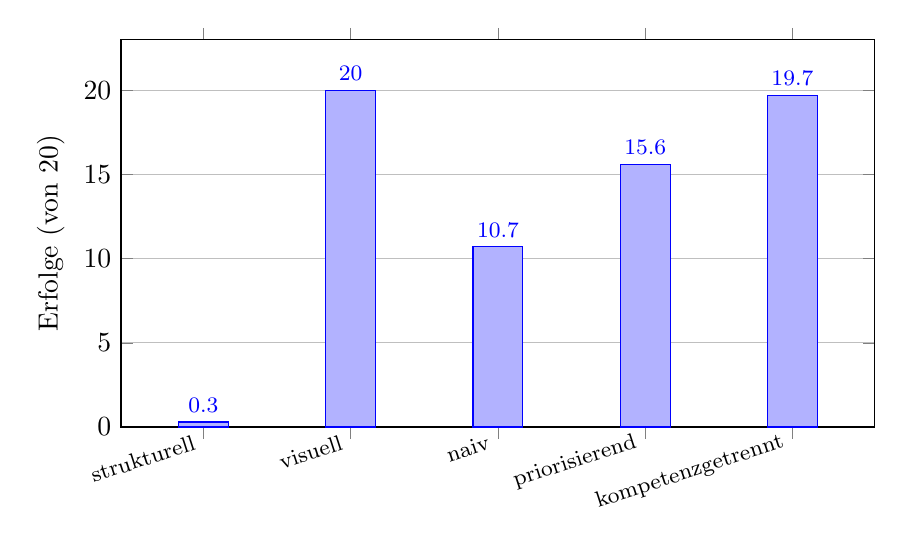
\begin{tikzpicture}
    \begin{axis}[
        ybar,
        width=0.92\linewidth,
        height=6.5cm,
        ymin=0, ymax=23,
        ytick={0,5,10,15,20},
        ylabel={Erfolge (von 20)},
        symbolic x coords={strukturell, visuell, naiv, priorisierend, kompetenzgetrennt},
        xtick=data,
        x tick label style={rotate=18, anchor=east, font=\footnotesize},
        nodes near coords,
        nodes near coords style={font=\footnotesize},
        bar width=18pt,
        enlarge x limits=0.14,
        ymajorgrids=true,
      ]
      \addplot coordinates {(strukturell,0.3) (visuell,20.0) (naiv,10.7) (priorisierend,15.6) (kompetenzgetrennt,19.7)};
    \end{axis}
  \end{tikzpicture}
  \caption{Erfolg in der rein visuellen Kategorie D über die fünf Varianten. Die rein visuelle Variante bildet die Obergrenze, die rein strukturelle scheitert nahezu vollständig. Die naive Kombination erreicht etwa die Hälfte, die Priorisierung verbessert das, und die Kompetenztrennung erreicht nahezu das Niveau der reinen Bildvariante.}
  \label{fig:kategorieD}
\end{figure}

\subsection*{Bewertung}

Gefordert war, dass eine Gestaltung dort belastbar verbessert, wo die naive Kombination scheitert, ohne in den übrigen Kategorien zu verlieren.
Die kompetenzgetrennte Variante erfüllt beides: Sie hebt D1 von 2 auf 29 von 30 Läufen und hält das Niveau in allen anderen gewerteten Kategorien.
Für dieses Szenarioset ist die zweite Forschungsfrage damit positiv beantwortet.
Die beiden Quellen ergänzen sich nicht von selbst, ihr Zusammenspiel lässt sich aber allein über die Instruktion steuern.
Einschränkend kommt hinzu, dass die Variante am Messset entwickelt wurde und Instruktion und Reihenfolge der Schichten nicht getrennt variiert sind; Abschnitt~\ref{sec:eval-validity} führt beides aus.

Als Leitlinie für einen lokalen Agenten mit gemischter Repräsentation lässt sich daraus ableiten, die Quellen nicht nur nebeneinanderzustellen, sondern jeder Schicht den Referenzbereich zuzuweisen, für den sie nach RQ1 exklusiv zuständig ist.
Die visuelle Beschreibung beantwortet dann, welches Objekt gemeint ist, die Struktur, wo es sich befindet.
Da diese Leitlinie auf zwei Szenarien einer Kategorie und einer an diesen Szenarien entwickelten Instruktion beruht, ist sie eine Empfehlung und kein nachgewiesenes Prinzip.
Die kompetenzgetrennte Variante bildet auch die Grundlage des Demonstrators aus Abschnitt~\ref{sec:impl-demonstrator}.


% ------------------------------------------------------------
\section{Validität und Grenzen}
\label{sec:eval-validity}

Die Ergebnisse sind nur so belastbar wie die Kontrolle der Bedingungen, unter denen sie entstanden.
Dieser Abschnitt beschreibt, welche Störfaktoren erkannt und beseitigt wurden, welche Einflüsse bestehen bleiben und wo die Aussagekraft endet.

\subsection*{Beseitigte Störfaktoren und nachträgliche Entscheidungen}

Mehrere zunächst plausible Befunde erwiesen sich bei genauerer Prüfung als Artefakte des Aufbaus und wurden vor der Wertung beseitigt.
Die Farbe der Marker beeinflusste die Farbwahrnehmung des visuellen Modells, das teils die Farbe des Markers statt die des Objekts nannte; die Marker wurden daraufhin versetzt und die Anweisung angepasst.
In Szenarien, in denen ein Referenzobjekt im Koordinatenursprung stand, fielen relative und absolute Zielangabe zusammen, sodass eine relationale Aufgabe auch ohne Verständnis der Relation lösbar war; diese Aufbauten wurden entkonfundiert.
Im ursprünglichen, achsenkollinearen Aufbau von C2 erhielten verdeckte Objekte durch den Sichtbarkeitstest keinen Marker, wodurch das kameranächste Objekt als einziges markiert erschien und die Aufgabe trivial wurde; C2 wurde mit seitlich versetztem Aufbau neu gemessen.
Ein scheinbar deutlicher Nachteil der hybriden Varianten schließlich entpuppte sich als Terminierungsartefakt des Frameworks und verschwand mit dem serverseitigen Schutz gegen identische Wiederholungen (Abschnitt~\ref{sec:impl-agent}).

Dass alle Varianten in der Kontrollkategorie A das Maximum erreichen, zeigt, dass der Messaufbau selbst keine variantenspezifischen Unterschiede erzeugt.
Vollständigkeit lässt sich daraus nicht ableiten: Die genannten Störfaktoren sind die markantesten, nicht notwendigerweise die einzigen.

Einige dieser Eingriffe erfolgten erst, nachdem die zugehörigen Ergebnisse vorlagen.
C3 wurde aus der Auswertung genommen, weil die achsenparallele Kameraausrichtung die aus Sicht der Kamera formulierte Referenz mehrdeutig machte; C2 wurde wegen des oben beschriebenen Markerproblems nicht ausgeschlossen, sondern mit verändertem Aufbau neu gemessen; und E2 wurde als nicht wertbar eingestuft, weil sein Soll-Ergebnis der Grundinstruktion widerspricht, was beim Entwurf nicht bedacht worden war.
In allen drei Fällen lag ein benennbarer Störfaktor vor, nicht bloß ein unerwünschtes Ergebnis.
Vorab festgelegt waren die Entscheidungen aber nicht, und ein solches Vorgehen erhöht grundsätzlich das Risiko, dass die berichtete Auswahl zugunsten der erzählten Deutung ausfällt.

% [INFO BENOETIGT] Ergebnisse der urspruenglichen Fassungen von C2 und C3
% Falls die Messwerte der ersten, spaeter verworfenen Fassungen von C2
% (achsenkollinearer Aufbau) und C3 noch vorliegen, sollten sie im Anhang
% vollstaendig berichtet werden. Das waere der wirksamste Beleg dafuer,
% dass die Ausschluesse sachlich und nicht ergebnisgetrieben erfolgten.
% Falls die Werte nicht mehr vorliegen, bitte hier vermerken, dass die
% Szenarien gemessen wurden, ihre Werte aber nicht erhalten sind.

\subsection*{Abhängigkeit vom Szenarioset}

An zwei Stellen sind die Testfälle in den Aufbau selbst eingeflossen.
Die erste ist der Wahrnehmungs-Prompt (Listing~\ref{lst:vlmprompt}).
Er bestimmt, was die visuelle Schicht überhaupt berichten kann, und begrenzt damit, was sich über ihre Schwächen sagen lässt.
Das Scheitern in B3 geht darauf zurück, dass der Prompt keine Größe abfragt; Kategorie B zeigt deshalb nicht, dass Attributreferenzen grundsätzlich strukturelle Daten erfordern, sondern nur, dass sie es unter diesem Prompt tun.
Umgekehrt nennt der Prompt als Beispiel für einen Texturdeskriptor \enquote{striped}, also das Merkmal, über das D1 und D2 ihr Zielobjekt ansprechen.
Weil alle Varianten mit visueller Schicht denselben Prompt nutzen, verzerrt das den Vergleich \emph{zwischen} ihnen nicht.
Gezeigt ist in Kategorie D aber nur, dass die visuelle Schicht eine Eigenschaft erkennt, auf die ihr Prompt sie ausdrücklich hinweist; ob sie ein unerwartetes Oberflächenmerkmal ebenso zuverlässig berichtet hätte, ist offen.

Die zweite und gewichtigere Stelle betrifft die kompetenzgetrennte Variante.
Sie entstand nicht aus einer vorab formulierten Theorie, sondern aus der Analyse der naiven und der priorisierenden Variante auf demselben Szenarioset, auf dem sie danach gemessen wird, und ihre Instruktion enthält mit \enquote{striped} und \enquote{most salient} zwei Formulierungen aus den Befehlen von D1 und D2 (Listing~\ref{lst:surgical}).
Gezeigt ist damit, dass sich die Kombination beider Schichten auf diesem Set durch die Instruktion erheblich verbessern lässt.
Nicht gezeigt ist, dass die Variante bei ungesehenen Formulierungen ebenso überlegen wäre.
Ein Teil ihres Vorteils könnte darauf beruhen, dass die Instruktion die Wörter des Testbefehls schon enthält und dem Modell die Zuordnung abnimmt, statt eine allgemeine Kompetenz zu vermitteln.
Zwischen beiden Möglichkeiten kann die Arbeit nicht entscheiden; Abschnitt~\ref{sec:zus-ausblick} nennt die Prüfungen, die dafür nötig wären.

\subsection*{Nicht getrennte Einflussgrößen}

Die hybriden Varianten unterscheiden sich nicht nur in ihrer Zuständigkeitsregel.
Die priorisierende stellt zusätzlich die visuelle Beschreibung voran, während die naive und die kompetenzgetrennte mit dem strukturellen Zustand beginnen (Tabelle~\ref{tab:variants}).
Instruktion und Reihenfolge variieren damit gemeinsam, und ihr jeweiliger Beitrag lässt sich nicht trennen.
Für den Vergleich der hybriden Varianten untereinander ist NFA5 insoweit nicht erfüllt; für den Vergleich von strukturell, visuell und hybrid gilt sie, da sich diese Bedingungen in der Repräsentation selbst unterscheiden.

Ungeklärt bleibt auch, warum die naive Kombination den Zugriff auf die visuelle Beschreibung in D1 verliert.
Formulierung des Befehls, visuelle Eindeutigkeit des Zielobjekts und Reihenfolge der Objekte (Abschnitt~\ref{sec:eval-rq2}) sind mit den Daten verträglich und lassen sich in diesem Aufbau nicht voneinander trennen.
Besonders schwer wiegt der Reihenfolgeeffekt, weil er nicht nur den Mechanismus, sondern den Befund selbst betrifft: Das Scheitern der strukturellen Variante mit 0 von 30 passt zu einer Positionspräferenz ebenso gut wie zu einer Verdrängung.
Die Deutung, die exakte strukturelle Information verdränge die unschärfere Beschreibung, ist deshalb eine mögliche Erklärung und kein nachgewiesener Mechanismus.
Die Ähnlichkeit zu Befunden über die Übergewichtung von Text in multimodalen Modellen~\cite{deng2025, wu2025} stützt sie nicht, denn dort konkurrieren Bild und Text innerhalb eines Modells, hier zwei Textquellen (Abschnitt~\ref{sec:grundlagen-sota}).

Ein weiterer Konflikt besteht zwischen der Grundinstruktion und den Mehrobjekt-Szenarien.
Die Grundinstruktion verlangt einen einzigen Manipulationsaufruf, die Soll-Ergebnisse von B2 und E2 betreffen aber mehrere Objekte.
Für E2 macht das die Zelle unwertbar, weil ein Erfolg nur durch Missachtung der Instruktion möglich ist.
Warum B2 den hybriden Varianten trotzdem durchgängig gelingt, ist ungeklärt und hängt davon ab, ob das Löschwerkzeug mehrere Objekte in einem Aufruf annimmt.
Damit bleibt auch offen, ob das knappe Kontextfenster von 4096 Token, das die hybriden Varianten stärker belastet (Abschnitt~\ref{sec:eval-design}), irgendwo wirksam wurde.
Für E2 läge diese Erklärung nahe, B2 spricht aber dagegen, und eine Protokollierung der Kontextauslastung je Lauf, die das klären könnte, wurde nicht vorgenommen.

\subsection*{Messung und Auswertung}

Der Erfolg wird ausschließlich aus dem Folgezustand bestimmt, weil das lokale Modell ein instabiles Abschlussverhalten zeigte.
Es meldete wiederholt Erfolge, die der Folgezustand nicht bestätigte, nannte teils nicht vorhandene Objektkennungen und führte einzelne Manipulationen doppelt aus.
Wie häufig Selbstauskunft und Folgezustand auseinanderfielen, wurde nicht quantifiziert; die Beobachtung beruht auf wiederholten Einzelfällen in den Protokollen.
Für die Gültigkeit der Ergebnisse genügt das, weil ein falsch gemeldeter Erfolg die Erfolgszahl nicht beeinflusst.

Innerhalb einer festen Konfiguration erwies sich die Messung als stabil.
Die meisten Zellen zeigen über die drei Durchläufe eine Spanne von null oder eins, nennenswerte Streuung tritt nur in wenigen Szenarien auf, vor allem in C1 und C4 sowie in D1 und D2 der priorisierenden Variante.
Wie in Abschnitt~\ref{sec:eval-design} ausgeführt, kommt diese Stabilität trotz einer Temperatur von 0{,}8 zustande.
Die Spannen dienen nur noch der Beschreibung der Durchlaufstabilität; die in einer früheren Fassung verwendete Heuristik, nicht überlappende Spannen als belastbaren Unterschied zu werten, wurde durch die Auswertung aus Abschnitt~\ref{sec:eval-metrics} ersetzt.

Die Konfidenzintervalle in Tabelle~\ref{tab:stats} quantifizieren allerdings nur die Unsicherheit innerhalb einer Zelle, nicht die Frage, ob diese Zelle für ihren Referenztyp repräsentativ ist.
Diese zweite Unsicherheit ist die größere und lässt sich hier nicht quantifizieren.
Den bild-exklusiven Bereich belegen zwei Szenarien, den strukturell-exklusiven nach dem Ausschluss von E2 nur eines, und das erlaubt keine Aussage darüber, wie sich der Effekt über die Breite möglicher Referenzen verhält.

Auch die Aufzeichnung der Läufe begrenzt die Analyse.
Für C2 und C4 liegen keine verwertbaren Protokolle mehr vor, sodass sich weder der Lagefehler bestimmen noch nachvollziehen lässt, welches Objekt der Agent in C2 tatsächlich manipuliert hat (Abschnitt~\ref{sec:eval-rq1}).
Werkzeugaufrufe mit Argumenten und erreichte Endpositionen mitzuschreiben, hätte keinen zusätzlichen Messaufwand bedeutet und mehrere der offenen Fragen dieser Arbeit beantwortet; bei einer Wiederholung ist das vorzusehen.
Schließlich wurde nicht geprüft, wie empfindlich insbesondere C2 und C4 auf die Toleranz $\tau = 0{,}1$ reagieren.
Eine großzügigere Toleranz könnte die dortigen Erfolgsraten anheben, ohne dass sich die Rangfolge der Varianten ändern muss.

\subsection*{Technische Einschränkungen}

Die Sichtbarkeitsprüfung arbeitet mit einem einzelnen Sichtstrahl auf den Objektmittelpunkt und kennt nur sichtbar und verdeckt (Abschnitt~\ref{sec:impl-scene}).
Für die verwendeten Szenen genügt das, in dichteren Szenen mit Teilverdeckung nicht.
Der Schutz gegen identische Wiederholungen würde auch eine vom Befehl geforderte Wiederholung blockieren (Abschnitt~\ref{sec:impl-agent}); in den ausgewerteten Szenarien kommt das nicht vor, bei Mehrschritt-Befehlen wäre es aber möglich.

\subsection*{Reichweite}

Alle Befunde beruhen auf einem einzelnen lokalen Modellpaar und auf synthetischen Szenen aus einfachen Grundkörpern.
Innerhalb dieses Rahmens sind sie repliziert und intern konsistent, eine Übertragung auf größere oder anders gebaute Modelle und auf reale, komplexe Szenen wurde aber nicht geprüft.
Für RQ2 kommt hinzu, dass die beste Variante am Szenarioset selbst entwickelt wurde.

Ein Teil der Befunde betrifft eher das Modell als die Repräsentation.
Für C4 ist die Deutung als Präzisionsgrenze tragfähig, denn die Koordinaten liegen vor, die geforderte Rechengenauigkeit wird aber nur manchmal erreicht, und daran ändert keine Repräsentation etwas.
Für C2 ist eine Modellgrenze dagegen nicht belegt (Abschnitt~\ref{sec:eval-rq1}).
C2 enthält zudem mit \enquote{nearest to the camera} eine blickpunktbezogene Referenz; dass blickpunktabhängige Referenzen nicht ausgewertet wurden, gilt also nur für das dafür vorgesehene und ausgeschlossene Szenario C3.

Die Aussagekraft der Arbeit liegt damit in der kontrollierten Isolation der Repräsentationskompetenzen und nicht in einer allgemeinen Gültigkeit über Modelle und Szenen hinweg.
